% F1: TWT mechanism timeline (two stations, SPs on a shared grid)
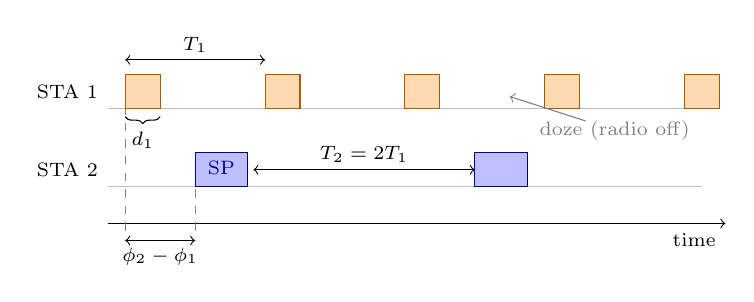
\begin{tikzpicture}[xscale=0.74, yscale=0.62, font=\scriptsize]
  % time axis
  \draw[->] (0,0) -- (10.6,0) node[below left] {time};

  % station 2 (period 2T): row at y=1
  \node[left] at (0,1.1) {STA 2};
  \draw[gray!50] (0,0.75) -- (10.2,0.75);
  \foreach \x in {1.5, 6.3} {
    \fill[blue!25] (\x,0.75) rectangle (\x+0.9,1.45);
    \draw[blue!60!black] (\x,0.75) rectangle (\x+0.9,1.45);
  }
  \node[blue!60!black] at (1.95,1.13) {SP};
  \draw[<->] (2.5,1.1) -- (6.3,1.1) node[midway, above=-1pt] {$T_2 = 2T_1$};

  % station 1 (period T): row at y=2.6
  \node[left] at (0,2.7) {STA 1};
  \draw[gray!50] (0,2.35) -- (10.2,2.35);
  \foreach \x in {0.3, 2.7, 5.1, 7.5, 9.9} {
    \fill[orange!30] (\x,2.35) rectangle (\x+0.6,3.05);
    \draw[orange!70!black] (\x,2.35) rectangle (\x+0.6,3.05);
  }
  \draw[<->] (0.3,3.35) -- (2.7,3.35) node[midway, above=-1pt] {$T_1$};
  \draw[decorate,decoration={brace,mirror,raise=2pt}] (0.3,2.3) -- (0.9,2.3)
    node[midway, below=4pt] {$d_1$};

  % doze annotation (between STA 1 SPs)
  \node[gray] at (8.7,1.9) {doze (radio off)};
  \draw[gray,->] (8.2,2.1) -- (6.9,2.6);

  % offset annotation
  \draw[dashed, gray] (0.3,-0.15) -- (0.3,2.35);
  \draw[dashed, gray] (1.5,-0.15) -- (1.5,0.75);
  \draw[<->] (0.3,-0.35) -- (1.5,-0.35) node[midway, below=-1pt] {$\phi_2 - \phi_1$};
\end{tikzpicture}
